\section{Introduction}

Cox proportional hazards regression \citep{cox1972regression} is a popular method for survival analysis, in which the response is the time to an event, typically a failure time. The main idea of Cox regression is that the predictors have a multiplicative effect on the hazard function. Meanwhile, the shape of the baseline hazard function is left unspecified and assumed to be the same for every subject. Estimation is based on a partial likelihood that considers only the ranks of the failure times, thereby producing a semiparametric method in which the effect of features on relative risk is modeled without assuming a distribution for the failure times. As a result Cox regression is more flexible and robust than parametric survival models, an appealing property since the distribution of failure times is often too complicated for simple parametric models. Cox regression is widely used in many domains including biostatistics, economics, and social science.

However, when the number of features is large, Cox regression, like other regression methods, is prone to over-fitting. Moreover, when the number of features is greater then number of events, the maximum likelihood estimates are no longer unique. Finally, coefficients go to infinity in the case of complete or quasi-complete separation, an event that is increasingly likely to occur as the number of features increase. Regularization methods such as the lasso are effective at dealing with all of these problems \citep{tibshirani1997lasso}. Lasso penalized Cox regression is not only more stable, but carries out automatic feature selection by setting many coefficients equal to zero, and is thus particularly attractive when dealing with high dimensional data. Typical practice is to solve the regression models over a path of decreasing values of the regularization parameter. Efficient algorithms for obtaining the solution path to lasso penalized Cox regression have been previously developed \citep{simon2011regularization}.

In recent years, big data has become more easily accessible and there is an increasing need to study ultra high dimensional data with millions of features. This introduces considerable challenges to existing optimization methods. One promising technique to tackle this challenge is ``screening'', in which ``inactive'' features -- features whose coefficients are equal to zero -- are identified prior to fitting and ``discarded''. The discarded features can then be ignored during the optimization, which results in dimension reduction and improvements in computation time and memory cost. The ``strong'' screening rule \citep{Tibshirani2012} was derived in a general form for a class of lasso type problems and the specific applications to lasso penalized Cox regression are also studies \citep{simon2011regularization,yang2013}. It discards a large proportion of features but requires a check afterwards to verify that no features were incorrectly discarded. Another type of screening is ``safe'' rules, which are mathematically guaranteed not to make a mistake and therefore don't require a check. Skipping the post-convergence checking stage saves time in general; however, safe rules are typically less powerful than strong rules in the sense of discarding fewer features, and which of the two approaches is best in practice depends on a number of factors, as investigated in \citep{Zeng2021}. For lasso penalized Cox regression, the only safe rule that we are aware of is SAFE \citep{ko2017solving}. However, this work is unpublished and there is a mistake in its derivation which makes it unsafe in the presence of tied failure times. Meanwhile, when there are no tied failure times, the SAFE rule is rather weak and discards only a small portion of features (if any).

A more powerful class of safe rules takes advantage of the path structure of the solution by utilizing solutions at previous penalty parameter values, thereby greatly increasing the number of features which can be discarded. Sequential screening can be carried out with such safe rules by always utilizing the previous solution in the path. Moreover, adaptive screening approaches \citep{wang2021adaptive} can also use such safe rules: a previous solution can be safely reused multiple times to greatly reduce the computation cost of screening at minimal cost in terms of screening power. Safe rules that utilize previous solutions are both mathematically and computationally more complicated and previous studies have focused almost exclusively on linear regression \citep{wang2013lasso}. A rare exception is the SLORES rule for lasso penalized logistic regression \citep{wang2014safe}, which was first proposed in a manner that does not consider previous solutions but can be extended to utilize previous solutions. This suggests the possibility of extending sequential safe rules to other types of lasso problems and incorporating them into an adaptive screening framework.

In this paper, we develop a novel safe rule for lasso penalized Cox regression that uses previous solutions to improve power. It is based on the dual form of the Cox partial likelihood; by deriving a bound for the dual solution, the rule can identify solutions whose primal coefficients will equal zero without actually solving the primal problem. The power of the proposed rule depends on the tightness of this bound and we discuss conditions under which the screening method is most and least powerful. Finally, we carry out numerical studies to show the advantages and disadvantages of the proposed rule.

\section{Screening Method}
\subsection{Problem Definition}

In a survival analysis, we collect data on $n$ subjects of the form $\{(t_i,y_i,\tilde{x}_i)\}_{i=1}^n$, where $t_i$ is the observed time on study and represents the time of failure if $y_i=1$ or the time of right censoring if $y_i=0$ (i.e., the failure happens at some unknown time after $t_i$), and $\tilde{x}_i=(X_{i1},X_{i2},...,X_{ip})$ is a vector of $p$ features. With these observed data, we can define the following quantities. Let $X=[\tilde{x}_1,\tilde{x}_2,...,\tilde{x}_n]^T=[x_1,x_2,...,x_p]$ denote the $n\times p$ feature matrix. Suppose there are $f$ unique times when at least one failure happens. Let  $\Delta=[\Delta_1,\Delta_2,...,\Delta_f]^T=\{\delta_{ki}\}\in\{0,1\}^{f\times n}$ denote the at-risk matrix, where $\delta_{ki}=1$ if subject $i$ is at risk at the $k$-th unique failure time. Let $Y$ denote the $f\times n$ response matrix where $Y_{ki}=1$ if subject $i$ died at the $k$-th unique failure time and $Y_{ki}=0$ otherwise. Finally, letting $y$ denote the $n \times 1$ response vector of elements $y_i$ and $d$ the $n \times 1$ vector of elements $d_k>0$, where $d_k$ denotes the number of failures at unique failure time $k$, we have $y=Y^T\mathbf{1}$ and $d=Y\mathbf{1}$.

The lasso penalized Cox regression, with the Breslow approximation \citep{breslow1974covariance} for tied failure times, consists of the optimization problem
\begin{equation}
    \label{eq:cox}
    \underset{\beta\in \mathbb{R}^p}{\mathrm{min}}-y^TX\beta+\sum_{k=1}^f d_k\log\left(\sum_{i=1}^n \delta_{ki} e^{\tilde{x}_i^T\beta}\right)+n\lambda||\beta||_1,
\end{equation}
where $\beta\in\mathbb{R}^p$ is the coefficient vector corresponding to the $p$ features and $\lambda>0$ is the regularization parameter that controls the size of lasso penalty. A dual form of \eqref{eq:cox} is given by (see Appendix~\ref{sec:dualcox} for details):
\begin{gather}
        \label{eq:dualTheta}
        \underset{\Theta\in \mathbb{R}^{f\times n}}{\mathrm{min}}g(\Theta)\equiv\sum_{k=1}^f\sum_{i=1}^n\delta_{ki}(Y_{ki}+d_k^{1/2}\Theta_{ki})\log\left(\frac{Y_{ki}}{d_k}+\frac{\Theta_{ki}}{d_k^{1/2}}\right)\\
        \begin{aligned}s.t.\quad \Theta\in \mathcal{F}_\lambda\equiv\{\Theta:\quad
            &||X^T\Theta^Td^{1/2}||_\infty\leq n\lambda,\quad D^{1/2}\Theta+Y+(1-\Delta)> 0,\\& \Theta\circ(1-\Delta)=0,\quad \Theta\mathbf{1}=0\}\nonumber,
        \end{aligned}
\end{gather}
where $\Theta\in \mathbb{R}^{f\times n}$ is the dual variable, $D=\textrm{diag}(d)$, ``$>$'' is element wise greater-than, $(\cdot)^{1/2}$ is the element wise square root, $\circ$ is element wise product, and we define $0\log 0$ to be 0. The dual problem therefore consists of minimizing the convex function $g(\Theta)$ within a convex feasible set $\mathcal{F}_\lambda$. Letting $\beta_\lambda$ denote the solution to the primal problem at penalty parameter value $\lambda$ and $\Theta_{\lambda}$ denote the corresponding dual solution, the primal solution and dual solution are connected by
\begin{equation}
    \label{eq:dualprimalcox}
    [\Theta_\lambda]_{ki}=d_k^{1/2}\delta_{ki}\frac{e^{\tilde{x}_i\beta_\lambda}}{\sum_{i'=1}^n\delta_{ki'}e^{\tilde{x}_{i'}\beta_\lambda}}-d_k^{-1/2}Y_{ki},
\end{equation}
for all $k$ and $i$. Furthermore, the KKT conditions for the primal problem~\eqref{eq:cox} can be expressed as:
\begin{gather}
    \label{eq:kktcox}
    \begin{aligned}&[\beta_\lambda]_{j}=0\implies\left|x_j^T\Theta_\lambda^Td^{1/2}\right|\leq n\lambda\\
    & [\beta_\lambda]_{j}\neq0\implies x_j^T\Theta_\lambda^Td^{1/2}= n\lambda\textit{sign}([\beta_\lambda]_{j}).
    \end{aligned}
\end{gather}
for any $j$. Combining \eqref{eq:dualprimalcox} and \eqref{eq:kktcox}, we can obtain a closed form solution for the problem at large $\lambda$ values:
\begin{gather}
    \label{eq:lammax}
    \begin{aligned}
        \beta_\lambda=0\iff \lambda \geq \lambda_{\max}&\equiv \max_j \left|x_j^T\Theta^T_{\lambda_{\max}}d^{1/2}\right|/n,\\
        \textrm{where}\quad[\Theta_{\lambda_{\max}}]_{ki}&=\frac{d_k^{1/2}\delta_{ki}}{\sum_{i'=1}^n\delta_{ki'}}-d_k^{-1/2}Y_{ki}.
    \end{aligned}
\end{gather}
Thus, when solving the problems on a grid of $L+1$ decreasing $\lambda$ values: $\lambda_0>\lambda_1>...>\lambda_L>0$, it makes more sense to choose $\lambda_0=\lambda_{\max}$ to take advantage of the known solution. If an algorithm solves the problems sequentially in decreasing order of $\lambda$, then the solution at $\lambda_{l'}$ will be known before solving the problem at $\lambda_l$ if $l'<l$. In the rest of this section, we will derive a screening method for this pathwise approach. Also, without loss of generality, we will derive the screening method for the problem at $\lambda_1$ assuming the solution at $\lambda_0$ is known and can be used as a reference for screening. We refer to this pair as the \quotes{target} ($\lambda_1)$ and the \quotes{reference} ($\lambda_0$). The same method can be applied to any pair of $\lambda_{l}$ and $\lambda_{l'}$. For simplicity, we will use $\beta_l,\Theta_l$ to denote the solution, and $\mathcal{F}_l$ to denote the feasible set, at any $\lambda_l$.

An important implication of the KKT conditions \eqref{eq:kktcox} is that for any $\lambda_1$, if 
\begin{equation}
    \label{eq:disc_condcox}
    |x_j^T\Theta_{1}^Td^{1/2}|<n\lambda_1,
\end{equation}
then we can safely conclude $[\beta_1]_{j}=0$ and the corresponding $x_j$ can be discarded from the optimization at $\lambda_1$. Although the left hand side of \eqref{eq:disc_condcox} is unknown until the solution is obtained, we can use the solution at $\lambda_{0}$ to derive a bound for the left hand side: $T_j(\lambda_{1},\lambda_{0};\Theta_{0})\geq |x_j^T\Theta_{1}^Td^{1/2}|$. Then, if $T_j(\lambda_{1},\lambda_{0};\Theta_{0})<n\lambda_1$ we can also safely conclude $[\beta_1]_{j}=0$. To achieve the greatest improvement in speed, $T_j(\lambda_{1},\lambda_{0};\Theta_{0})$ should be as small as possible, as this will result in the greatest number of discarded features.

\subsection{Dual Variable Bound}

The only unknown term in \eqref{eq:disc_condcox} is $\Theta_{1}$. In this section we will derive a bound for $\Theta_{1}$ assuming the previous solution $\Theta_{0}$ is known.

\begin{lemma}
    \label{lem:1}
    For any $0<\lambda_1<\lambda_0$, $\mathcal{F}_{1}\subseteq\mathcal{F}_{0}$.
\end{lemma}

The lemma also implies that $\mathcal{F}_{1}\subseteq\mathcal{F}_{\infty}\equiv\{\Theta: D^{1/2}\Theta+Y+(1-\Delta)> 0,\Theta\circ(1-\Delta)=0, \Theta\mathbf{1}=0\}$.

The dual function $g(\Theta)$ is twice differentiable in $\mathcal{F}_{\infty}$, so by its second order expansion we have:
\begin{equation}
        \label{eq:expand}
        g(\Theta_{1})-g(\Theta_{0})-\langle\nabla g(\Theta_{0}),\Theta_{1}-\Theta_{0}\rangle=\frac{1}{2}\langle\nabla^2 g(\Theta''),(\Theta_{1}-\Theta_{0})^{\circ 2}\rangle,%\geq \frac{1}{2}||\Theta'-\Theta||_2^2,
\end{equation}
for any $\lambda_1<\lambda_{0}\in (0,\lambda_\textrm{max}]$, where $(\cdot)^{\circ2}$ is element-wise square, $\langle A,B\rangle=\sum_{i=1}^n\sum_{i'=1}^mA_{ii'}B_{ii'}$ for any $n\times m$ matrices $A$ and $B$, and $\Theta''$ is some point on the line segment between $\Theta_{1}$ and $\Theta_{0}$. Because $\Theta_{1}$ and $\Theta_{0}$ are in the convex set $\mathcal{F}_{0}$, $\Theta''$ is also in $\mathcal{F}_{0}$ and thus in $\mathcal{F}_{\infty}$. Note that
\begin{align*}
  [\nabla g(\Theta'')]_{ki} &= \delta_{ki}d_k^{1/2}\log\left(\frac{Y_{ki}}{d_k}+\frac{\Theta''_{ki}}{d_k^{1/2}}\right)+d_k^{1/2} \\
  [\nabla^2 g(\Theta'')]_{ki,ki} &= \frac{\delta_{ki}d_k}{Y_{ki}+d_k^{1/2}\Theta''_{ki}},
\end{align*}
and $\nabla^2 g(\Theta'')$ is a diagonal matrix. For convenience, we will instead use $[\nabla^2 g(\Theta'')]$ to denote the $f\times n$ matrix where $[\nabla^2 g(\Theta'')]_{ki}=\frac{\delta_{ki}d_k}{y_{ki}+d_k^{1/2}\Theta''_{ki}}$. Using this expansion, we can derive a bound for $\Theta_{1}$.
\begin{theorem}
    \label{thm:1}
    For any $\lambda_1<\lambda_{0}\in (0,\lambda_\textnormal{max}]$ 
    \begin{equation}
        \left\langle\nabla^2 g(\Theta''),\left(\Theta_{1}-\frac{\lambda_1}{\lambda_0}\Theta_{0}\right)^{\circ 2}\right\rangle\leq r^2(\lambda_1,\lambda_0)\equiv 2\left(g\left(\frac{\lambda_1}{\lambda_0}\Theta_{0}\right)-g*\right),
    \end{equation}
    for some $\Theta''\in\mathcal{F}_{\infty}$ and any $g^*\leq g(\Theta_{1})$.
\end{theorem}

An obvious choice of $g^*$ is $g(\Theta_{0})$ since
\begin{equation*}
  g(\Theta_{1}) = \underset{\Theta\in \mathcal{F}_{1}}{\mathrm{min}}g(\Theta)\geq\underset{\Theta\in \mathcal{F}_{0}}{\mathrm{min}}g(\Theta) = g\left(\Theta_{0}\right).
\end{equation*}
We propose to instead use $g^* = g(\Theta^*_{1})$, where
\begin{gather}
    \label{eq:gstar}
    \begin{aligned}
        &g(\Theta^*_{1}) \equiv \min_\Theta g(\Theta)\\
        s.t.\quad &|x_j^T\Theta d^{1/2}|\leq n\lambda_1,\forall j:|x_j^T\Theta_{0} d^{1/2}|= n\lambda_0,\\&D^{1/2}\Theta+Y+(1-\Delta)> 0, \Theta\circ(1-\Delta)=0,\quad \Theta\mathbf{1}=0.
    \end{aligned}
\end{gather}
Note that $g(\Theta^*_{1}) \leq g(\Theta_{1})$ because compared to $\mathcal{F}_{1}$, the problem in \eqref{eq:gstar} has fewer constraints and its feasible set contains $\mathcal{F}_{1}$. Problem \eqref{eq:gstar} is also easy to optimize since it is equivalent to optimizing the primal problem with only features $x_j$ that satisfy $|x_j^T\Theta_{0} d^{1/2}|= n\lambda_0$, or in other words, have non-zero coefficients at $\lambda_0$. Due to the sparsity of lasso solutions, only a small number of features will be included and the primal problem can be optimized quickly. After solving the primal problem, $\Theta_1^*$ and thus $g(\Theta_1^*)$ can be easily computed by \eqref{eq:dualprimalcox}. Moreover, the primal solution can be used as a warm start for optimization at $\lambda_1$, so solving for $g(\Theta^*_{1})$ will not introduce extra cost. \pb{Is this true? It is not obvious to me that \eqref{eq:dualprimalcox} can be easily solved for $\beta$ in terms of $\Theta$ and therefore that one can use the solution to the dual problem as a warm start.}

Theorem \ref{thm:1} says $\Theta_{1}$ is bounded within an ellipsoid centered at $\frac{\lambda_1}{\lambda_0}\Theta_{0}$, with shape controlled by $\nabla^2g(\Theta'')$ and size controlled by $r(\lambda_1,\lambda_0)$. Note that the center and the size do not involve the unknown quantity $\Theta_{1}$. Because $d_k^{1/2}\Theta''_{ki}+y_{ki}\geq 0$ and $\sum_{i=1}^nd_k^{1/2}\Theta''_{ki}+y_{ki}=d_k$, we have $d_k^{1/2}\Theta''_{ki}+y_{ki}\leq d_k$ and $[\nabla^2 g(\Theta'')]_{ki}\geq\delta_{ki}\geq 0$, so $g(\Theta)$ is convex. Furthermore, $\forall\Theta,\Theta'\in\mathcal{F}_{\infty}$, if $\delta_{ki}=0$, $\Theta_{ki}=\Theta'_{ki}=0$, so in $\mathcal{F}_{\infty}$, $g(\Theta)$ is actually strongly convex with $[\nabla^2 g(\Theta)]_{ki}\geq 1$ if $\delta_{ki}=1$. This implies the bound in Theorem \ref{thm:1} is a proper ellipsoid in the subspace $\mathcal{F}_{\infty}$, although the $\Theta''$ that controls its shape is unknown.

\subsection{Upper bound via Solving Bounded Optimization}

In this section, we derive the upper bound $T_j(\lambda_1,\lambda_0;\Theta_{0})$ for $|x_j^T\Theta^T_{1}d^{1/2}|$ using the bound in Theorem~\ref{thm:1} and the fact that $\Theta''\in\mathcal{F}_{\infty}$.

If $\Theta''$ were known, then by Theorem~\ref{thm:1} and the fact that $\Theta_{1}$ is in the feasible set $\mathcal{F}_{1}$, $\Theta_{1}$ is bounded in the convex compact set
 \begin{equation}
     \mathcal{A}(\lambda_1,{\lambda_0},\Theta'')\equiv\{\Theta:\langle\nabla^2 g(\Theta''),(\Theta-\Theta_{0})^{\circ 2}\rangle\leq r^2(\lambda_1,\lambda_0),\,\Theta\circ(1-\Delta)=0,\, \Theta\mathbf{1}=0\}.
 \end{equation}
Now, $|x_j^T\Theta^T_{1}d^{1/2}|$ is bounded above by:
\begin{equation}
    T^*_{j}(\lambda_1,\lambda_0;\Theta_{0},\Theta'')\equiv\max_{\Theta\in\mathcal{A}(\lambda_1,{\lambda_0},\Theta'')} |x_j^T\Theta^T d^{1/2}|;
\end{equation}
this problem is equivalent to the maximum of the 2 sub-problems:
\begin{equation}
    \label{eq:bounddual}
    T^*_{\xi,j}(\lambda_1,\lambda_0;\Theta_{0},\Theta'')\equiv\max_{\Theta\in\mathcal{A}(\lambda_1,\lambda_0,\Theta'')} \xi x_j^T\Theta^T d^{1/2},
\end{equation}
where $\xi = \pm 1$. Before deriving an upper bound for $T^*_{\xi,j}(\lambda_1,\lambda_0;\Theta_{0},\Theta'')$, we first establish two supporting lemmas.

\begin{lemma}
    \label{lem:2}
    For any $\lambda_1<\lambda_{0}\in (0,\lambda_\textnormal{max}]$, strong duality holds for \eqref{eq:bounddual} and an optimal solution is admitted in $\mathcal{A}(\lambda,{\lambda_0},\Theta'')$.
\end{lemma}

Lemma~\ref{lem:2} says that the solution to \eqref{eq:bounddual} is the same as its dual solution, given in Lemma~\ref{lem:3}. \comment{This does not sound correct. Primal and dual problems solve for different variables. It is the maximum and minimum that are the same.}

\begin{lemma}
    \label{lem:3}
    Denote
    \begin{equation}
        \label{eq:w}
        W_{ki}\equiv\delta_{ki}\frac{Y_{ki}+d_k^{1/2}\Theta_{ki}''}{d_k},
    \end{equation}
    with $W$ being the $f\times n$ matrix of $W_{ki}$ and $W_k$ being the $k$-th row of $W$.\\
    If $P_{\mathbf{1}}x_j\neq 0$, the maximum in \eqref{eq:bounddual} is equal to:
    \begin{equation}
        \label{eq:tstar}
        T^*_{\xi,j}(\lambda_1,\lambda_0;\Theta_{0},\Theta'')=\frac{\lambda_1}{\lambda_0}\xi x_j^T\Theta_{0}^Td^{1/2}+r(\lambda_1,\lambda_0)\sqrt{\sum_{k=1}^fd_k\sum_{i=1}^nW_{ki}\left(X_{ij}-W_k^Tx_j\right)^2},
    \end{equation}
    where $P_{\mathbf{1}}$ is the projection matrix onto $\mathbf{1}$.
\end{lemma}

The condition $P_{\mathbf{1}}x_j \ne 0$ simply means that $X_{ij}$ is not constant across all subjects. This assumption can be made without loss of generality, since features that violate this assumption do not contain any information. Unfortunately, $T^*_{\xi,j}(\lambda,\lambda_0;\Theta_{0},\Theta'')$ still contains an unknown quantity, since $W$ depends on $\Theta''$. Thus, we again use the fact $\Theta''\in\mathcal{F}_\infty$ to construct an upper bound for $T^*_{\xi,j}(\lambda,\lambda_0;\Theta_{0},\Theta'')$ that does not depend on $\Theta''$.

\begin{theorem}
    \label{thm:2}
    Let
    \begin{equation}
        \label{eq:prod}
        ||x||_\psi\equiv\sqrt{\sum_{k=1}^f\frac{d_k}{4}\left(\max_{i:\delta_{ki}=1}x_i-\min_{i:\delta_{ki}=1}x_i\right)^2}.
    \end{equation}
    If $P_{\mathbf{1}}x_j\neq 0$,
    \begin{equation}
        \label{eq:gbbar}
        \xi x_j^T\Theta_{1}d^{1/2}\leq T^*_{\xi,j}(\lambda_1,\lambda_0;\Theta_{0},\Theta'')\leq T_{\xi,j}(\lambda_1,\lambda_0;\Theta_{0})\equiv\frac{\lambda_1}{\lambda_0}\xi x_j^T\Theta_{0}^Td^{1/2}+r(\lambda_1,\lambda_0)||x_j||_\psi.
    \end{equation}
\end{theorem}

With this result, we finally arrive at an upper bound,

\begin{equation}
    \label{eq:bound}
    T_j(\lambda_1,\lambda_0;\Theta_{0})\equiv\max_{\xi=-1,1}\{T_{\xi,j}(\lambda_1,\lambda_0;\Theta_{0})\}=\frac{\lambda_1}{\lambda_0}\left| x_j^T\Theta_{0}^Td^{1/2}\right|+r(\lambda_1,\lambda_0)||x_j||_\psi,
\end{equation}
for $|x_j^T\Theta^T_{1}d^{1/2}|$ that does not depend on any unknown quantities. 

\subsection{Safe Screening Rule of lasso Penalized Cox Regression}

Theorem~\ref{thm:2} and \eqref{eq:bound} imply that for any $j$ and pair of points on a solution path $l^*<l$, if $T_j(\lambda_{l},\lambda_{l^*};\Theta_{l^*})<n\lambda_l$ then we can safely conclude $[\beta_l]_{j}=0$ and $x_j$ can be removed from the optimization at $\lambda_l$. We formally present this safe screening method, which can be used in combination with any optimization algorithm for lasso penalized Cox regression, in the following algorithm.

\begin{algorithm}[H]
    \SetKwInOut{Input}{Input}\SetKwInOut{Output}{Output}\SetKwInOut{Pre}{Pre-compute}\SetKwInOut{Initialize}{Initialize}\SetKwInOut{Choose}{Choose}
    \Input{$X,Y,\Delta$, $\lambda_0=\lambda_{\max}>\lambda_1>...>\lambda_L>0$}
    \Initialize{$\beta_{0} = 0$}

    
    \For{$l\xleftarrow{}$ 1 \KwTo L}{
        \Initialize{$\mathcal{A}_l=\{1,2,...,p\}$}
        \Choose{$l^*<l$}
        \For{$j\xleftarrow{}$ 1 \KwTo p}{
            \uIf{$T_j(\lambda_l,\lambda_{l^*};\Theta_{l^*})<n\lambda_l$}{
                Remove $j$ from $\mathcal{A}_l$\;
            }
        }
        Run any optimization algorithm for lasso penalized Cox regression problem with input: $X_{\mathcal{A}_l},Y,\Delta,\lambda_l$. Save the solution $\beta_{l}$.
    }
    \Output{$\{\beta_{l}\}_{l=0}^L$}
\end{algorithm}

The $X_{\mathcal{A}_l}$ in the algorithm above denotes the sub-matrix of $X$ where the $j$-th column of $X$ is contained if and only if $j\in{\mathcal{A}_l}$. Any optimization algorithm can benefit from having a reduced input feature matrix $X_{\mathcal{A}_l}$. For example, the time cost of coordinate descent algorithm for lasso penalized Cox regression \citep{simon2011regularization} is roughly linear with the size of $\mathcal{A}_l$. Although the screening method is proposed for a sequence of $\lambda$ values, it can also be applied to solve the problem at a single $\lambda$ value by considering the sequence with length 2: $\lambda_{\max},\lambda$, since the solution at $\lambda_{\max}$ always has a simple closed form.

The algorithm presented here can be used for sequential screening, in which one always uses the latest previous solution, by always setting $l^*$ to be $l-1$ over the entire solution path. A more efficient approach, however, is adaptive screening, which reuses the same value of $l^*$ multiple times to reduce computation costs and waits until it is beneficial to choose a new value. Adaptive screening is described in detail in \citep{wang2021adaptive}.

\section{Experiments}

In this section, we will use simulated data to evaluate the performance of the sequential version of the proposed safe method for lasso penalized Cox regression. The experiment on the sequential version eliminates other factors that can impact the performance and better illustrates the properties of the proposed safe rule. The data is simulated from the model: for each subject $i\in\{1,2,...,n\}$, $t_i\sim \lfloor\max\{Weibull(\exp(\tilde{x}_i\beta),2), 5\}/c\rfloor $, independent of $y_i\sim binary(0.7)$ and subjects are independent. $\beta$ is a vector of $p$ coefficients with $s$ of them uniformly distributed between $(-b,b)$ and $p-s$ of them being $0$. Elements of $X$ are first simulated i.i.d from $Beta(\alpha,\alpha)$ and then standardized column-wise. The lasso penalized Cox regression is solved along a path of $L$ $\lambda$ values equally spaced on log scale between $(\lambda_{\min},\lambda_{\max})$, where $\lambda_{\max}$ is determined by the data according to \eqref{eq:lammax}. 

By default, we set $n=1,000$, $p=3,000$, $c=0.5$, $s=10$, $b=1$, $\alpha=0.2$, $L=100$ and $\lambda_{\min}=0.05\lambda_{\max}$. In each experiment, one of the factors will vary and the performance will be compared in terms of the total power, which is defined as the total number of discards along the path over the total number of 0 coefficients along the path. We will use the experiment to study the how the factors affect the screening power and what are the limitations of the proposed screening method.

\subsection{Limitations}
\label{sec:lim}


The nature of Cox regression is very different from other generalized linear regression problems. This leads to some limitations when developing sequential safe rule for lasso penalized Cox regression and thus a weaker screening power. In this section we will discuss some limitations that prevent us from developing a powerful screening. By understanding the limitations, we will show under some special cases, the proposed method have a much better performance.


For a general class of lasso penalized convex problems, the problem can be defined as:
\begin{equation}
    \underset{\beta,\beta_0\in \mathbb{R}^p}{\mathrm{min}}l(X\beta+x_0^T\beta_0)+n\lambda||\beta||_1,
\end{equation}
where $l$ is closed convex twice differentiable function, $x_0$ is a known vector and $\beta_0$ is an unpenalized coefficient. Standard lasso, lasso penalized Cox regression, lasso penalized Logistic regression and a number of lasso type problems can all be expressed as the form above. One simple definition of the dual form is:
\begin{gather}
    \begin{aligned}
         \underset{\theta\in \mathbb{R}^n}{\mathrm{min}} g(\theta)\quad s.t.\quad x_0^T\theta=0,||X^T\theta||_\infty\leq n\lambda
    \end{aligned}
\end{gather}
where $g(\theta)=\max_z \theta^Tz-l(z)$ is the conjugate of $l$, which is also convex and $\theta$ is the $n$-dimensional dual variable.

If $l$ can be written as sum of independent terms: $l(X\beta+x_0^T\beta_0)=\sum_i l_0(\tilde{x}_i^T\beta+x_{0i}\beta_0)$, then the dual function can be written as sum of independent univariate maximization problems: $g(\theta)=\sum_i\max_{z_i} \theta_iz_i-l_0(z_i)$. It is easier to obtain a closed form solution for such univariate problems and thus a closed form for dual function $g$. For example, a closed form can be obtained for standard lasso and lasso penalized Logistic regression. After a closed form is obtained, we can look at its second order expansion to find an $n$-dimensional ellipsoid bound for the dual variable.

For problems like Cox regression, $l$ cannot be written as sum of independent terms and finding $g$ becomes an $n$-variate maximization problems. It is hard to obtain a closed form solution. A numeric solution would be too expensive and outweighs the gain a screening could bring. To overcome this problem, we have to use a more complicated dual problem \eqref{eq:dualTheta}, which involves a $n\times f$-dimensional dual variable. 

\subsubsection{Dimensionality of Dual Form}

Because we have an $n\times f$-dimensional dual variable, an ellipsoid bound for this dual variable will be much looser because of the dimensionality. The dual variable has more ``bad'' directions it can go to and leads to a much larger upper bound.

By this argument, it will be less of a problem when $f$ is smaller. It is a reasonable scenario in practice, for example, when the failure times are recorded in units of large intervals (months, years) and there are a lot of tied failure times and a small number of unique failure times. We consider the experiment where the length of the intervals $c$ vary and because the observed times are generated between the fixed range$(0,5)$, the maximum of number of unique observed times will be decreasing in $c$. Because the sample size is limited and some samples are censored, the number of unique failure times $f$ may not reach the maximum but should be decreasing as well. The following plot summarize the effect of $c$ and the maximum number of unique observed times, on the total screening power.

\begin{figure}[ht]
    \centering
    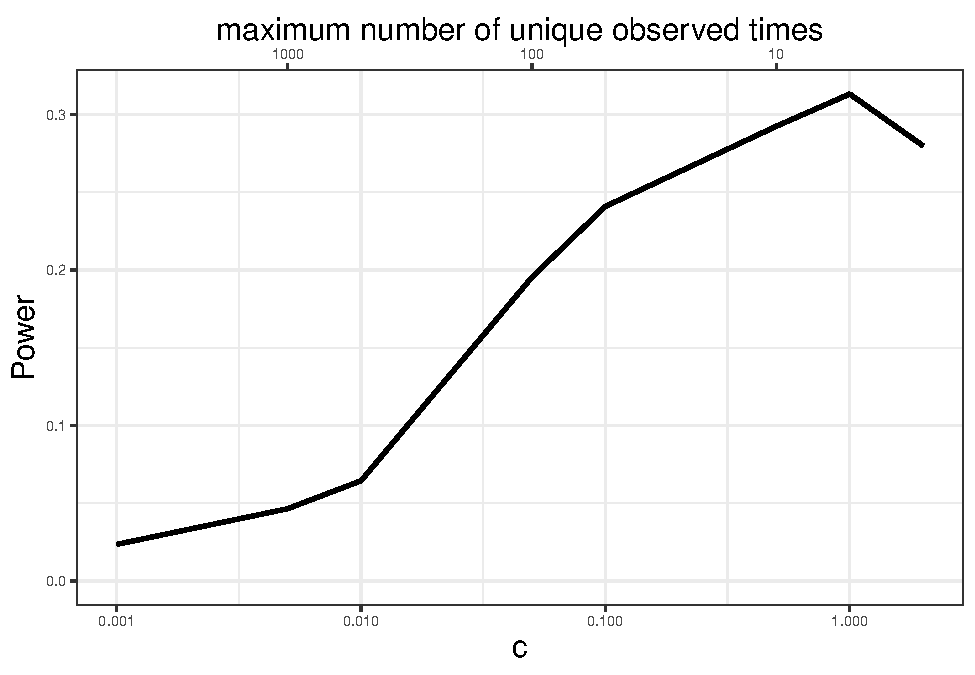
\includegraphics[width=0.6\textwidth]{interval.pdf}
    \caption{Average proportion of feature discarded along the path by interval length $c$ and maximum number of unique observed times}
\end{figure}

Note that as $c$ increases and the failure times are cut into less larger intervals, the information in failure times decreases and thus the signal-to-noise ratio decreases. From this aspect, we should expect the screening power to decrease. From the plot, the screening power mostly increases, as $c$ increases and $f$ decreases, and the result supports our argument. In the end when $c$ is too large, the loss in signal dominates and leads to a drop in screening power.

\subsubsection{Distribution of Features}

The high dimensionality of the dual problem not only gives more freedom to the dual solution $\Theta_\lambda$, but also gives more freedom to the variable $\Theta''$ in Theorem \ref{thm:1}, which controls the shape of the ellipsoid bound for $\Theta_\lambda$. $\Theta''$ has the freedom to go to a direction that leads to a ``bad'' shape. It is shown in the difference between Lemma \ref{lem:3}, where $\Theta''$ is assumed known, and Theorem \ref{thm:2}, where the worst $\Theta''$ is considered. The impact can be interpreted as substituting a weighted variance whose weights $W$ depends on $\Theta''$ and are somewhat evenly distributed, with a weighted variance who puts half weight on the two extremist points each. The ratio between these two terms can be expressed as:
\begin{equation}
    \label{eq:alpharatio}
    \frac{4\sum_{k=1}^fd_k\sum_{i=1}^nW_{ki}\left(X_{ij}-W_k^Tx_j\right)^2}{\sum_{k=1}^fd_k\left(\max_{i:\delta_{ki}=1}X_{ij}-\min_{i:\delta_{ki}=1}X_{ij}\right)^2}
\end{equation}

The case when the freedom of $\Theta''$ has a small impact will be the case when ratio between them is close to 1. It is also a reasonable scenario in practice. For example, when a variable is binary and nearly balanced, the ratio between the two variances will be close to 1. We consider the experiment where the parameter $\alpha$ vary. Elements of $X$ are generated from $Beta(\alpha,\alpha)$ which is bounded from two ends. A small value of $\alpha$ will put more weights on two ends and the distribution will resemble a balanced binary distribution, while a larger value of $\alpha$ will lead to a unimodal bell shaped distribution that increases the difference between two weighted variances. Each $x_j$ is also standardized to make sure the difference is not caused by the scale. The following plot summarize the effect of $\alpha$ on the total screening power. The ratio in \eqref{eq:alpharatio} is also computed.

\begin{figure}[ht]
    \centering
    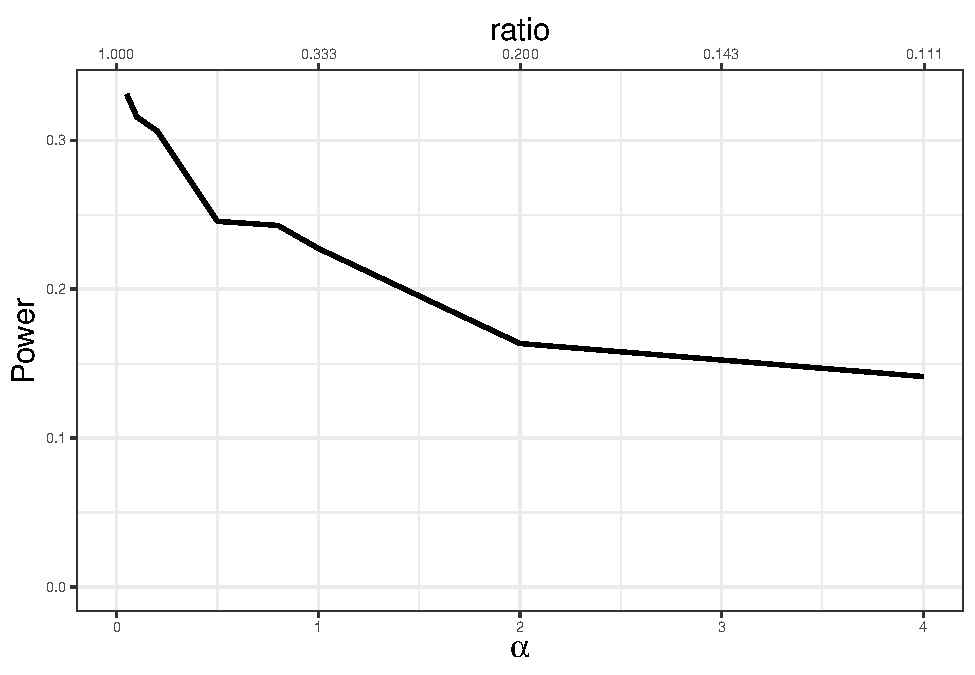
\includegraphics[width=0.6\textwidth]{alpha.pdf}  
    \caption{Average proportion of feature discarded along the path by shape $\alpha$ and ratio \eqref{eq:alpharatio}}
\end{figure}

The result shows that a distribution of $x_j$ that puts more weight on two ends (small $\alpha$) leads to much better performance, while a distribution of $x_j$ that puts more weight in the center (large $\alpha$) leads to worse performance.

\subsection{Other Common Factors}

In this section, we consider the experiments that study the effect of other common factors in the simulation. The result is summarized in the following plot.

\begin{figure}[ht]
    \centering
    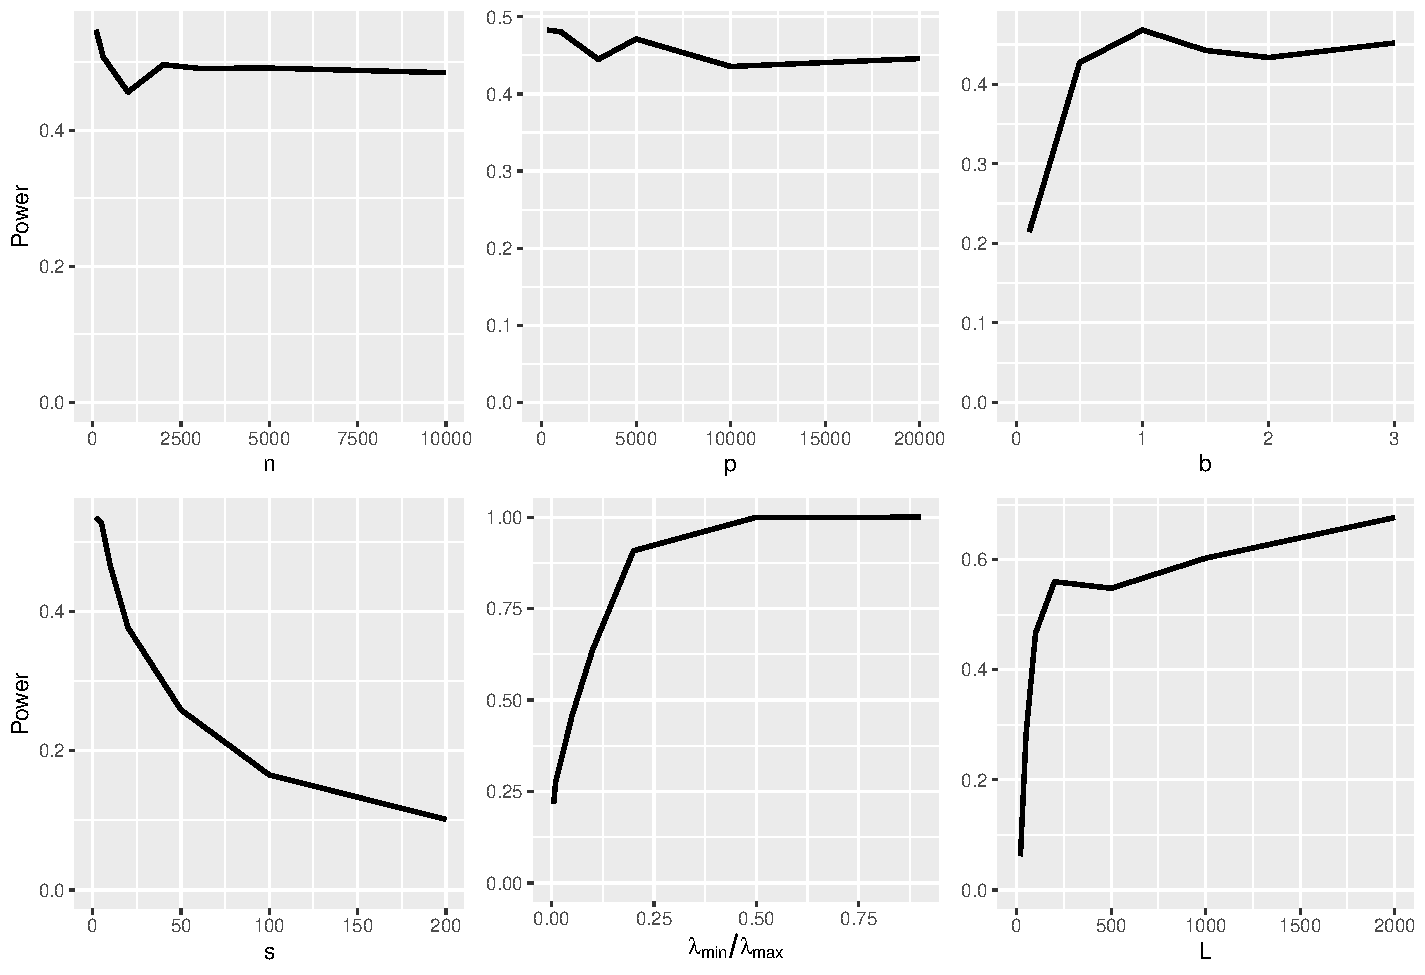
\includegraphics[width=\textwidth]{coxsim.pdf}    
    \caption{Average proportion of feature discarded along the path by common factors}
\end{figure}

On the first row, we vary the sample size $n$, the number of features $p$ and size of coefficients $b$ respectively. These factors does not have a significant impact on the performance, except in the extreme case when the $n$ or $b$ is extremely small and the signal in the data becomes too weak to provide useful information. On the second row, we first vary the number of nonzero coefficients $s$ and the screening methods performs better when $s$ is smaller, the underlying model is sparser and a lasso penalty is more appropriate. Second, we vary the ratio $\lambda_{\min}/\lambda_{\max}$. The screening method is more powerful when this ratio is larger, which leads to a solution path with sparser solutions and closer spaced $\lambda$ values. Closer spaced $\lambda$ values means that the previous solution will be closer to the current solution and thus will be more helpful for screening at current solution. Last, we vary the number of $\lambda$ values in the solution path and the screening method is more powerful when $L$ is larger, which means $\lambda$ values are spaced closer.  

\section{Application}

In this section, we will test the proposed sequential safe rule on the Lung Cancer Patients data \citep{shedden2008gene}, to help solve the lasso penalized Cox regression problem explaining lung cancer hazard with gene expression levels and some demographic data as features. The observed time $t_i$ is the number of months in study. The observed event is a failure ($y_i=1$) if the patient died. There are $p=22,304$ features in the feature matrix used to explain failure, with $22,283$ being gene expression levels and the rest $21$ being demographic features. The sample size is $n=442$. The lasso penalized Cox regression problem will be solved along a path of $L=100$ lambda values equally spaced on log scale between $(0.2\lambda_{\max},\lambda_{\max})$. 

To address the limitations discussed in \ref{sec:lim}, we will consider modified datasets combining the following two modifications on the raw data. First, we can cut the observed times into intervals of length 1 year. This modification reduce the number of unique failure times and reduce the dimensionality of the dual form. Second, we can cut each gene expression level feature at its sample median to create a binary feature. This modification leads to a balanced binary distribution of the features and tightens the ratio in \eqref{eq:alpharatio}. These two modification also represents special cases that can occur in real data. The first modification corresponds to survival data where observed times are recorded in coarse units. The second modification corresponds to data where features are recorded in levels of ``high'' and ``low'', instead of raw measurements.

In the following experiment, we will test different screening methods, and the algorithm optimizing the reduced problem after screening is the Coordinate Descent \citep{simon2011regularization} with Active Cycling \citep{lee2007efficient}. Active Cycling (AC) is a simple idea similar to screening, where the reduced problem with only features that are active in previous solution is first solved and then a KKT condition check validates if there is any other active feature. It is easy to be implemented with any screening method and is shown to greatly reduce computation cost in most cases, so in this experiment we combine it with all screening method. The screening methods we compare are: no screening other than AC (AC), basic version of the sequential safe rule that uses only the solution at $\lambda_{\max}$ (Basic), sequential safe rule that uses previous solution (Sequential), sequential strong rule (SSR) and adaptive screening built on the sequential safe rule (Adaptive).

Table \ref{Tab:realcox} summarizes the total computation cost with standard error in second, using different screening methods and datasets. In the dataset with coarse observed times and binary features (Both Modified), the sequential safe screening can provide significant speedup that is close to sequential strong rule. Moreover, an adaptive screening can be built upon the sequential safe rule and outperform all other screening methods in the special case. The adaptive screening method is also robust and is close to fastest under all cases.

\begin{table}[H]
\centering
\begin{tabular}{lllll}
\toprule
Screening method & Raw Data & Modified Times & Modified Features & Both Modified \\
\midrule
AC & 2.386 (0.003) & 1.889 (0.005) & 2.342 (0.004) & 1.869 (0.004) \\
Basic & 2.463 (0.003) & 1.919 (0.003) & 2.288 (0.004) & 1.906 (0.004) \\
Sequential & 2.911 (0.003) & 2.262 (0.004) & 2.447 (0.006) & 1.306 (0.005) \\
SSR & \textbf{1.254 (0.003)} & \textbf{1.055 (0.004)} & \textbf{1.225 (0.003)} & 1.030 (0.003) \\
Adaptive & 1.302 (0.004) & 1.078 (0.002) & 1.255 (0.003) & \textbf{0.769 (0.003)} \\
\bottomrule
\end{tabular}
\caption{Average computing time in second (standard error)}
\label{Tab:realcox}
\end{table}



The following plot shows the number of features discarded by sequential safe rule at each $\lambda$ value on each dataset. It shows that smaller number of unique failure times and distribution of features closer to balanced binary distribution both lead to stronger screening power of the sequential safe rule.

\begin{figure}[ht]
    \centering
    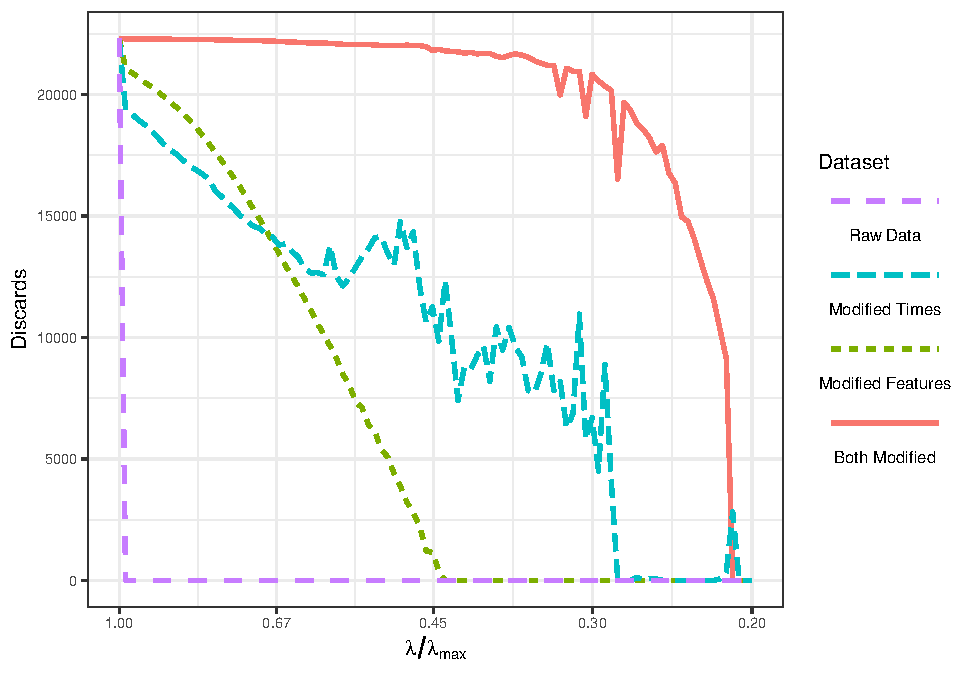
\includegraphics[width=0.7\textwidth]{shedden.pdf}    
    \caption{Number of discarded feature along the path on different modifications}
\end{figure}

\section{Discussion}

In this paper, we propose a novel safe screening rule to help solving lasso penalized Cox regression efficiently along a path of $\lambda$ values. It can utilize previous solutions on the path to discard much more features that will have 0 coefficients. \comment{The rule is derived by looking at an augmented dual problem and constructing a closed form upper bound for the inner product between features and dual variables}. We study factors that affect the power of the screening method and show that under some special cases it can discard a substantial proportion of features and can provide benefits in computation cost when incorporated into the adaptive screening framework. The results also show the possibility to derive a safe screening method that can utilize previous solution in the path, for lasso type problems with nonstandard likelihood functions that are not separable and can provide insights for developing screening methods for other lasso type problems.

\appendix
\appendixpage


\section{Derivation of the Dual Problem}
\label{sec:dualcox}

Introducing a new variable $Z\equiv\mathbf{1}\beta^TX^T\in\mathbb{R}^{f\times n}$, which means $z_{ki}\equiv\tilde{x}_i^T\beta,\,\forall k$, then the problem \eqref{eq:cox} becomes:
\begin{equation}
    \label{eq:dual+z}
    \begin{gathered}
    \underset{\beta\in \mathbb{R}^p}{\mathrm{min}}-y^TX\beta+\sum_{k=1}^f d_k\log\left(\sum_{i=1}^n \delta_{ki} e^{z_{ki}}\right)+n\lambda||\beta||_1\\s.t.\quad Z=\mathbf{1}\beta^TX^T.
\end{gathered}
\end{equation}

Let $\langle\cdot,\cdot\rangle$ denote the matrix element-wise inner product, where $\langle A,B \rangle\equiv\sum_{k=1}^f\sum_{i=1}^nA_{ki}B_{ki}$.

Introducing the dual variable $U\in\mathbb{R}^{f\times n}$, the dual problem becomes:
\begin{gather}
    \label{eq:dual+u}
    \begin{aligned}
        &\underset{U\in \mathbb{R}^{f\times n}}{\mathrm{max}}\underset{Z\in \mathbb{R}^{f\times n}}{\mathrm{min}}\underset{\beta\in \mathbb{R}^p}{\mathrm{min}}-y^TX\beta+\sum_{k=1}^f d_k\log\left(\sum_{i=1}^n \delta_{ki} e^{z_{ki}}\right)+n\lambda||\beta||_1+\langle U,\mathbf{1}\beta^TX^T-Z\rangle\\
        =&\underset{U\in \mathbb{R}^{f\times n}}{\mathrm{max}}\underset{Z\in \mathbb{R}^{f\times n}}{\mathrm{min}}\underset{\beta\in \mathbb{R}^p}{\mathrm{min}}-y^TX\beta+\sum_{k=1}^f d_k\log\left(\sum_{i=1}^n \delta_{ki} e^{z_{ki}}\right)+n\lambda||\beta||_1+\langle U,\mathbf{1}\beta^TX^T\rangle-\langle U,Z\rangle\\
        =&\underset{U\in \mathbb{R}^{f\times n}}{\mathrm{max}}\underset{Z\in \mathbb{R}^{f\times n}}{\mathrm{min}}\underset{\beta\in \mathbb{R}^p}{\mathrm{min}}-y^TX\beta+\sum_{k=1}^f d_k\log\left(\sum_{i=1}^n \delta_{ki} e^{z_{ki}}\right)+n\lambda||\beta||_1+\mathbf{1}^TUX\beta-\langle U,Z\rangle
    \end{aligned}    
\end{gather}
Minimizing with respect to $\beta$, the partial derivative is:
\begin{equation}
    \label{eq:partialbeta}
    \frac{\partial}{\partial\beta}(\cdot) =-X^Ty+X^TU^T\mathbf{1}+n\lambda\frac{\partial||\beta||_1}{\partial\beta}
\end{equation}
so the minimum is obtained iff $||X^TU^T\mathbf{1}-X^Ty||_\infty\leq n\lambda,$ and the problem becomes:
\begin{gather}
    \label{eq:dual-beta}
    \begin{aligned}
        &\underset{U\in \mathbb{R}^{f\times n}}{\mathrm{max}}\underset{Z\in \mathbb{R}^{f\times n}}{\mathrm{min}}- \langle U,Z\rangle+\sum_{k=1}^f d_k\log\left(\sum_{i=1}^n \delta_{ki} e^{z_{ki}}\right)\\
        =&\underset{U\in \mathbb{R}^{f\times n}}{\mathrm{max}}\underset{Z\in \mathbb{R}^{f\times n}}{\mathrm{min}}-\sum_{k=1}^f u_k^Tz_k +\sum_{k=1}^f d_k\log\left(\sum_{i=1}^n \delta_{ki} e^{z_{ki}}\right)\\
        =&\underset{U\in \mathbb{R}^{f\times n}}{\mathrm{max}}\sum_{k=1}^f\underset{z_k\in \mathbb{R}^n}{\mathrm{min}}-u_k^Tz_k+d_k\log\left(\sum_{i=1}^n \delta_{ki} e^{z_{ki}}\right)\\
        &s.t.\quad ||X^TU^T\mathbf{1}-X^Ty||_\infty\leq n\lambda.
    \end{aligned}
\end{gather}
Take derivative with respect to $z_{ki}$:
\begin{equation}
    \label{eq:partialz}
    \frac{\partial}{\partial z_{ki}}(\cdot)=-u_{ki}+\frac{d_k\delta_{ki}e^{z_{ki}}}{\sum_{i'=1}^n \delta_{ki'} e^{z_{ki'}}},
\end{equation}
and the minimum is obtained when $u_{ki}=\frac{d_k\delta_{ki}e^{z_{ki}}}{\sum_{i'=1}^n \delta_{ki'} e^{z_{ki'}}}$, which can be obtained iff:
\begin{gather}
    \label{eq:constu1}
    \begin{aligned}
    &u_{ki} > 0\textrm{ if }\delta_{ki}=1,\,\forall k,i\\
    &u_{ki}=0\textrm{ if }\delta_{ki}=0,\,\forall k,i\\
    &\sum_{i=1}^n u_{ki}=d_k,\,\forall k
\end{aligned}
\end{gather}
or
\begin{gather}
    \label{eq:constu2}
    \begin{aligned}
    &U+(1-\Delta)>0\\
    &U\circ(1-\Delta)=0\\
    &U\mathbf{1}=d
\end{aligned}
\end{gather}
where $>$ is hold element-wise and $\circ$ is element-wise product. The problem becomes
\begin{gather}
    \label{eq:dualu}
    \begin{aligned}
        &\underset{U\in \mathbb{R}^{f\times n}}{\mathrm{max}}-\sum_{k=1}^f\sum_{i=1}^n\delta_{ki}u_{ki}\log\left(\frac{u_{ki}\sum_{i'=1}^n \delta_{ki'} e^{z_{ki'}}}{d_k}\right)+\sum_{k=1}^fd_k\log\left(\sum_{i=1}^n \delta_{ki} e^{z_{ki}}\right)\\
        =&\underset{U\in \mathbb{R}^{f\times n}}{\mathrm{max}}-\sum_{k=1}^f\sum_{i=1}^nu_{ki}\log u_{ki}-\sum_{k=1}^f\sum_{i=1}^nu_{ki}\log\left(\sum_{i'=1}^n \delta_{ki'} e^{z_{ki'}}\right)+\sum_{k=1}^f\sum_{i=1}^nu_{ki}\log d_k+\sum_{k=1}^fd_k\log\left(\sum_{i=1}^n \delta_{ki} e^{z_{ki}}\right)\\
        =&\underset{U\in \mathbb{R}^{f\times n}}{\mathrm{max}}-\sum_{k=1}^f\sum_{i=1}^nu_{ki}\log\frac{u_{ki}}{d_k}\\
        =&\underset{U\in \mathbb{R}^{f\times n}}{\mathrm{min}}\sum_{k=1}^f\sum_{i=1}^n\delta_{ki}u_{ki}\log\frac{u_{ki}}{d_k}\\
        &s.t.\quad ||X^TU^T\mathbf{1}-X^Ty||_\infty\leq n\lambda,\quad U+(1-\Delta)>0,\quad U\circ(1-\Delta)=0,\quad U\mathbf{1}=d.
    \end{aligned}
\end{gather}

Let $d^{1/2}=\{d_k^{1/2}\}_{k=1}^f$ and $D^{1/2}=diag(d^{1/2})$. Note that \begin{itemize}
    \item $X^T(U^T-Y^T)D^{-1/2}d^{1/2}=X^T(U^T-Y^T)\mathbf{1}=X^TU^T\mathbf{1}-X^TY^T\mathbf{1}=X^TU^T\mathbf{1}-X^Ty$,
    \item $D^{1/2}D^{-1/2}(U-Y)+Y+(1-\Delta)=U+(1-\Delta)$,
    \item $\left(D^{-1/2}(U-Y)\right)\circ(1-\Delta)=D^{-1/2}\left((U-Y)\circ(1-\Delta)\right)=D^{-1/2}\left(U\circ(1-\Delta)\right)=0$ iff $U\circ(1-\Delta)=0$,
    \item $D^{-1/2}(U-Y)\mathbf{1}=D^{-1/2}(U\mathbf{1}-Y\mathbf{1})=D^{-1/2}(U\mathbf{1}-d)=0$ iff $U\mathbf{1}-d=0$.
\end{itemize}
Letting $\Theta=D^{-1/2}(U-Y)$, then the dual problem \eqref{eq:dualu} can be expressed as in \eqref{eq:dualTheta} and the dual solution and primal solution can be connected by \eqref{eq:dualprimalcox}.


\section{Proof of Theorem \ref{thm:1}}


It can be shown that $\frac{\lambda_1}{\lambda_0}\Theta_{0}\in\mathcal{F}_{1}$ because
\begin{itemize}
    \item $||X^T\frac{\lambda_1}{\lambda_0}\Theta_{0}^Td^{1/2}||_\infty=\frac{\lambda_1}{\lambda_0}||X^T\Theta_{0}^Td^{1/2}||_\infty\leq \frac{\lambda_1}{\lambda_0}n\lambda_0=n\lambda_1$.
    \item Each element in the inequality $D^{1/2}\Theta+Y+(1-\Delta)> 0$ is $d_k^{1/2}\Theta_{ki}+Y_{ki}+(1-\delta_{ki})>0$. Also, $Y_{ki}+(1-\delta_{ki})\geq 0$. If $[\Theta_0]_{ki}>0$, $d_k^{1/2}\frac{\lambda_1}{\lambda_0}[\Theta_0]_{ki}+Y_{ki}+(1-\delta_{ki})\geq d_k^{1/2}\frac{\lambda_1}{\lambda_0}[\Theta_0]_{ki}>0.$ If $[\Theta_0]_{ki}\leq0$, $d_k^{1/2}\frac{\lambda_1}{\lambda_0}[\Theta_0]_{ki}+Y_{ki}+(1-\delta_{ki})\geq d_k^{1/2}[\Theta_0]_{ki}+Y_{ki}+(1-\delta_{ki})>0.$
    \item Other constraints obviously hold.
\end{itemize}
Therefore $\Theta_{1},\frac{\lambda_1}{\lambda_0}\Theta_{0}\in \mathcal{F}_{1}$. Its second order expansion is:
\begin{equation}
    \label{eq:thm2.1}
    \left\langle\nabla^2 g(\Theta''),\left(\Theta_{1}-\frac{\lambda_1}{\lambda_0}\Theta_{0}\right)^{\circ 2}\right\rangle=2\left(g\left(\frac{\lambda_1}{\lambda_0}\Theta_{0}\right)-g(\Theta_{1})+\left\langle\nabla g\left(\Theta_{1}\right),\left(\Theta_{1}-\frac{\lambda_1}{\lambda_0}\Theta_{0}\right)\right\rangle\right),
\end{equation}
 for some $\Theta''\in[\Theta_1,\frac{\lambda}{\lambda_0}\Theta_{0}]\subseteq \mathcal{F}_\lambda$. Looking at the gradient term, the Slater's condition and thus the KKT condition for the dual problem \eqref{eq:dualTheta} holds at $\lambda_1$:
\begin{equation}
    \label{eq:thm2.3}
    0=[\nabla g(\Theta_{1})]_{ki}+\sum_{j=1}^p\eta^+_jX_{ij}d_k^{1/2}+\sum_{j=1}^p\eta^-_j(-X_{ij}d_k^{1/2})-\mu_{ki}d_k^{1/2}+\nu_{ki}(1-\delta_{ki})+\zeta_k,
\end{equation}
$\forall i,k$, where $\eta^+,\eta^-\in\mathbb{R}^p_+,\{\mu\}_{k,i}\in\mathbb{R}^{f\times n}_+,\{\nu\}_{k,i}\in\mathbb{R}^{f\times n},\zeta\in\mathbb{R}^f$ are vectors depending on $\lambda_0$. Because $\{D^{1/2}\Theta+Y+(1-\Delta)>0\}$ is an open set and $\Theta_{1}$ must be an interior point of it, by complementary slackness, $\mu_{ki}=0,\forall k,i$. Therefore, \eqref{eq:thm2.3} becomes $\forall i,k$:
\begin{equation}
    \label{eq:thm2.4}
    0=[\nabla g(\Theta_{1})]_{ki}+\sum_{j=1}^p\eta^+_jX_{ij}d_k^{1/2}+\sum_{j=1}^p\eta^-_j(-X_{ij}d_k^{1/2})+\nu_{ki}(1-\delta_{ki})+\zeta_k.
\end{equation}

By complementary slackness again, $\eta^+_j>0$ only if $x_j^T\Theta_{1}^Td^{1/2}=\sum_{i=1}^n\sum_{k=1}^fX_{ij}[\Theta_1]_{ki}d_k^{1/2}=n\lambda_1$ and $\eta^-_j>0$ only if $-x_j^T\Theta_{1}^Td^{1/2}=\sum_{i=1}^n\sum_{k=1}^f(-X_{ij}[\Theta_1]_{ki}d_k^{1/2})=n\lambda_1$. $\eta^+_j=\eta^-_j=0$ otherwise. Therefore:
\begin{gather}
    \label{eq:thm2.5}
    \begin{aligned}
        -\langle\nabla g(\Theta_{1}),\Theta_{1}\rangle&=\sum_{i=1}^n\sum_{k=1}^f-[\nabla g(\Theta_{1})]_{ki}[\Theta_1]_{ki}\\
        &=\sum_{j=1}^p\eta^+_j\sum_{i=1}^n\sum_{k=1}^fX_{ij}[\Theta_1]_{ki}d_k^{1/2}+\sum_{j=1}^p\eta^-_j\sum_{i=1}^n\sum_{k=1}^f(-X_{ij}[\Theta_1]_{ki}d_k^{1/2})\\
        &\quad+\sum_{i=1}^n\sum_{k=1}^f\nu_{ki}(1-\delta_{ki})[\Theta_1]_{ki}+\sum_{k=1}^f\zeta_{k}\sum_{i=1}^n[\Theta_1]_{ki}\\
        &=\sum_{j=1}^p\eta^+_j\sum_{i=1}^n\sum_{k=1}^fX_{ij}[\Theta_1]_{ki}d_k^{1/2}+\sum_{j=1}^p\eta^-_j\sum_{i=1}^n\sum_{k=1}^f(-X_{ij}[\Theta_1]_{ki}d_k^{1/2})\\
        &=\sum_{j:x_j^T\Theta_{1}^Td^{1/2}=n\lambda_1}n\lambda_1\eta_j^++\sum_{j:-x_j^T\Theta_{1}^Td^{1/2}=n\lambda_1}n\lambda_1\eta_j^-\\
        &=n\lambda_1\left(\sum_{j:x_j^T\Theta_{1}^Td^{1/2}=n\lambda_1}\eta_j^++\sum_{j:-x_j^T\Theta_{1}^Td^{1/2}=n\lambda_1}\eta_j^-\right),
    \end{aligned}
\end{gather}
where the third equation holds because $\Theta_{1}\in\mathcal{F}_{1}$.

Because $\frac{\lambda_1}{\lambda_0}\Theta_{0}\in \mathcal{F}_{1}$, $\left|x_j^T\frac{\lambda_1}{\lambda_0}\Theta_{0}^Td^{1/2}\right|=\left|\sum_{i=1}^n\sum_{k=1}^fX_{ij}\frac{\lambda_1}{\lambda_0}[\Theta_0]_{ki}d_k^{1/2}\right|\leq n\lambda_1$. Similarly:
\begin{gather}
    \label{eq:thm2.6}
    \begin{aligned}
        -\langle\nabla g(\Theta_{1}),\frac{\lambda_1}{\lambda_0}\Theta_{0}\rangle
        &=\sum_{j=1}^p\eta^+_j\sum_{i=1}^n\sum_{k=1}^fX_{ij}\frac{\lambda_1}{\lambda_0}[\Theta_0]_{ki}d_k^{1/2}+\sum_{j=1}^p\eta^-_j\sum_{i=1}^n\sum_{k=1}^f(-X_{ij}\frac{\lambda_1}{\lambda_0}[\Theta_0]_{ki}d_k^{1/2})\\
        &\leq\sum_{j:x_j^T\Theta_{1}^Td^{1/2}=n\lambda_1}n\lambda_1\eta_j^++\sum_{j:-x_j^T\Theta_{1}^Td^{1/2}=n\lambda_1}n\lambda_1\eta_j^-\\
        &=n\lambda_1\left(\sum_{j:x_j^T\Theta_{1}^Td^{1/2}=n\lambda_1}\eta_j^++\sum_{j:-x_j^T\Theta_{1}^Td^{1/2}=n\lambda_1}\eta_j^-\right)\\
        &=-\langle\nabla g(\Theta_{1}),\Theta_{1}\rangle.
    \end{aligned}
\end{gather}

Combining \eqref{eq:thm2.1}, \eqref{eq:thm2.5}, \eqref{eq:thm2.6} and any $g^*\leq g(\Theta_{1})$, we have Theorem~\ref{thm:1} holds and end the proof.

\hspace{0 in}

\section{Proof of Lemma \ref{lem:2}}

To show the strong duality of \eqref{eq:bounddual}, we are going to show the Slater's condition holds. The objective function and all constraints in $\mathcal{A}(\lambda_1,{\lambda_0},\Theta'')$ except for $\langle\nabla^2 g(\Theta''),(\Theta-\Theta_{0})^{\circ 2}\rangle\leq r^2(\lambda_1,\lambda_0)$ are linear. The objective function and all constraints are convex. $\Theta_{0}$ is a value of $\Theta$ in $\mathcal{A}(\lambda_1,{\lambda_0},\Theta'')$ that satisfies the strict inequality $\langle\nabla^2 g(\Theta''),(\Theta-\Theta_{0})^{\circ 2}\rangle=0< r^2(\lambda_1,\lambda_0)$. The Slater's condition and thus the strong duality holds.

Also, the objective function is continuous and $\mathcal{A}(\lambda_1,{\lambda_0},\Theta'')$ is compact, so an optimal solution will be admitted in $\mathcal{A}(\lambda,{\lambda_0},\Theta'')$.


\section{Proof of Lemma \ref{lem:3}}

The Lagrangian of negative of \eqref{eq:bounddual} is:
\begin{gather}
    \label{eq:lem4.1}
    \begin{aligned}
        L(\Theta,u,V_1,v_2)=&-\xi x_j^T\Theta^T d^{1/2}+\frac{u}{2}\left(\langle\nabla^2 g(\Theta''),(\Theta-\frac{\lambda_1}{\lambda_0}\Theta_{0})^{\circ 2}\rangle-r^2(\lambda_1,\lambda_0)\right)
        +\langle V_1,\Theta\circ(1-\Delta)\rangle+v_2^T\Theta\mathbf{1}\\
        =&\left\langle\left(-\xi d^{1/2}x_j^T+V_1\circ(1-\Delta)+v_2\mathbf{1}^T\right),\Theta\right\rangle+\frac{u}{2}\left(\langle\nabla^2 g(\Theta''),(\Theta-\frac{\lambda_1}{\lambda_0}\Theta_{0})^{\circ 2}\rangle-r^2(\lambda_1,\lambda_0)\right)
    \end{aligned}
\end{gather}
where $u\geq 0$, $V_1\in\mathbb{R}^{f\times n},v_2\in\mathbb{R}^f$ are Lagrangian multipliers. Because of strong duality of \eqref{eq:bounddual}, $-T_{\xi,j}(\lambda,\lambda_0;\Theta_{0},\Theta'')$ is equal to the maximization of \eqref{eq:lem4.1}. Take derivative with respect to $\Theta$ and set to 0:

\begin{equation}
    \label{eq:lem4.2}
    \nabla_\Theta L(\Theta,u,V_1,v_2)=-\xi d^{1/2}x_j^T+u\nabla^2g(\Theta'')\circ(\Theta-\frac{\lambda_1}{\lambda_0}\Theta_{0})+V_1\circ(1-\Delta)+v_2\mathbf{1}^T=0.
\end{equation}

\begin{enumerate}
    \item When $u\neq 0$, because $\Theta_{ki},[\Theta_0]_{ki}\neq0\implies W_{ki}[\nabla^2g(\Theta'')]_{ki}=\delta_{ki}=1$ we have:
    \begin{equation}
        \label{eq:lem4.3}
        \Theta=\frac{\lambda_1}{\lambda_0}\Theta_{0}-\frac{1}{u}W\circ\left(-\xi d^{1/2}x_j^T+V_1\circ(1-\Delta)+v_2\mathbf{1}^T\right).
    \end{equation}

    Combining \eqref{eq:lem4.1},\eqref{eq:lem4.3} and the fact that $\Theta_{0}\in\mathcal{F}_{0}$, the dual function $\bar{g}(u,V_1,v_2)\equiv\min_\Theta L(\Theta,u,V_1,v_2)$ is:
    \begin{equation}
    \label{eq:lem4.4}
    \tilde{g}(u,V_1,v_2)=-\frac{\lambda_1}{\lambda_0}\xi x_j^T\Theta_{0}^Td^{1/2}-\frac{1}{2u}\left\langle W,\left( -\xi d^{1/2} x_j^T+V_1\circ(1-\Delta)+v_2\mathbf{1}^T\right)^{\circ2}\right\rangle-\frac{1}{2}ur(\lambda_1,\lambda_0)^2.
    \end{equation}

    The dual problem is to maximize the dual function under $u> 0$. It is unconstrained with respect to $V_1,v_2$. Take derivative with respect to $V_1,v_2$ and set to 0:

    \begin{equation}
        \label{eq:lem4.5}
        \begin{cases}
        \frac{\partial}{\partial V_1}=-\frac{1}{u}W\circ(1-\Delta)\circ\left(-\xi d^{1/2} x_j^T+V_1\circ(1-\Delta)+v_2\mathbf{1}^T\right)=0,\\
        \frac{\partial}{\partial v_2}=-\frac{1}{u}W\circ\left( -\xi d^{1/2} x_j^T+V_1\circ(1-\Delta)+v_2\mathbf{1}^T\right)\mathbf{1}=0.
        \end{cases}
    \end{equation}
    The first equation is automatically satisfied because the constraint $W\circ(1-\Delta)=0$. Note in \eqref{eq:lem4.4}, if $\delta_{ki}=1$, $[V_1\circ(1-\Delta)]_{ki}=0$ and if $\delta_{ki}=0$, $W_{ki}=0$, so $V_1\circ(1-\Delta)$ can be set to 0 without changing the value of $\tilde{g}(u,V_1,v_2)$.

    The second equation states that each row of the matrix $W\circ\left( -\xi d^{1/2} x_j^T+v_2\mathbf{1}^T\right)$ sums to 0, or in other word, each row of $W\circ\left(-\xi d^{1/2}x_j^T\right)$ is centered.

    Combining \eqref{eq:lem4.4} and \eqref{eq:lem4.5} the dual problem becomes maximizing $\bar{g}(u)=\max_{V_1,v_2}\tilde{g}(u,V_1,v2)$ under constrains $u>0$. It is also easy to see that $\Theta''\in\mathcal{F}_{0}\implies\sum_{i=1}^nW_{ki}=1,\forall k$. $W_k$ is a proper vector of weights, so we have
    \begin{equation}
        \label{eq:lem4.6}
        \bar{g}(u)=-\frac{\lambda_1}{\lambda_0}\xi x_j^T\Theta_{0}^Td^{1/2}-\frac{1}{2}ur^2(\lambda_1,\lambda_0)-\frac{1}{2u}\sum_{k=1}^fd_k\sum_{i=1}^nW_{ki}\left(X_{ij}-W_k^Tx_j\right)^2.
    \end{equation}
    Both $r^2(\lambda_1,\lambda_0)$ and $\sum_{k=1}^fd_k\sum_{i=1}^nW_{ki}\left(X_{ij}-W_k^Tx_j\right)^2$ are non-negative, so the maximum is easy to obtain, and negative of the maximum will be the maximum in \eqref{eq:tstar}.

    \item When $u=0$, to solve \eqref{eq:lem4.2} we need to solve $-\xi d^{1/2} x_j^T+V_1\circ(1-\Delta)+v_2\mathbf{1}^T=0.$ At the first unique failure time $k_0\in\{1,2,3,...,f\}$, all the subjects are at risk and $\delta_{k_0,i}=1,\forall i$. With out loss of generality, assume $k_0=1$. The first row of this equation becomes:

    \begin{equation}
        -\xi d_1^{1/2}x_j + v_{2,1}\mathbf{1}=0.
    \end{equation}

    Let $P_{\mathbf{1}}=I_n-\mathbf{1_n}\mathbf{1_n}^T$ be the projection onto the orthogonal complement of the space spanned by $\mathbf{1}$. Multiply both sides by $-\xi d^{-1/2}_1P_{\mathbf{1_n}}$ we have:

    \begin{equation}
        \label{eq:lem4.7}
        P_{\mathbf{1}}x_j=0,
    \end{equation}
    which means $x_j$ is a vector of a constant and contradicts the assumption. Thus $-\xi d^{1/2} x_j^T+V_1\circ(1-\Delta)+v_2\mathbf{1}^T\neq0.$ $\tilde{g}(0,V_1,v2)\equiv\min_\Theta L(\Theta,0,V_1,v_2)=-\infty$ because $L(\Theta,0,u_2,V_1,v_2)$ is linear in $\Theta$ with nonzero coefficients. End of proof.


\end{enumerate}


\section{Proof of Theorem \ref{thm:2}}

    Let $V_{w}(x)\equiv\sum_{i=1}^nw_{i}\left(x_i-w^Tx\right)^2$ denote the weighted variance of $x$ with weights $w$.\\
    In \eqref{eq:tstar}, we can see that the term $\sum_{i=1}^nW_{ki}\left( X_{ij}-W_k^Tx_j\right)^2=V_{W_k}(x_j)$ is the weighted variance of $x_j$ with weight $W_k$ because $\Theta''\in\mathcal{F}_{0}\implies\sum_{i=1}^nW_{ki}=1$. Because $\Theta''\in\mathcal{F}_{0}$, another constraint is $W_{ki}=0$ if $\delta_{ki}=0$. The weighted variance will be maximized when the two extremist points each have $\frac{1}{2}$ weight:
    \begin{equation}
        \label{eq:lem5.2}
        V_{W_k}(x_j)\leq \frac{\left(\max_{i:\delta_{ki}=1}X_{ij}-\min_{i:\delta_{ki}=1}X_{ij}\right)^2}{4},
    \end{equation}
    which holds for all $x_j$. Plugging\eqref{eq:lem5.2} into $T^*_{\xi,j}(\lambda_1,\lambda_0;\Theta_{0},\Theta'')$ in \eqref{eq:tstar} finishes the proof.







